\section{Background}
\label{sec:Background}

\subsection{Messages}
\label{sub:Messages}

In today's interconnected world, computer programs rarely exist in a vacuum.
Rather, they form one small part of a much larger \gls{soa} -
consisting of multiple services, jobs and scripts, all exchanging information in
the form of messages. These messages may adhere to a standard data-interchange
format (for example, \gls{json}). They may correspond to an agreed upon
specification (for example, \href{https://goo.gl/rjuP4C}{IEEE 1671-2010}).
Or they may simply be blobs of binary information transmitted over the network -
completely subject to the interpretation of the sender and received.
At a fundamental level, though, a message is simply a collection of bytes, to be
transmitted from point A, to point B.

\subsection{Message Brokers}
\label{sub:What is a message broker?}

\begin{figure}[ht]
  \centering
  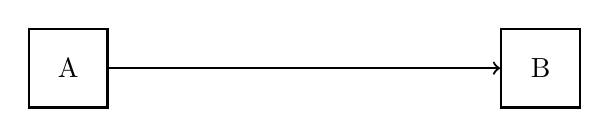
\begin{tikzpicture}[thick]
  \node(A) [draw,rectangle,minimum width=1cm,minimum height=1cm]{A};

  \begin{scope}[xshift=6cm]
    \node(B) [draw,rectangle,minimum width=1cm,minimum height=1cm]{B};
  \end{scope}

  \draw[->] (A) edge (B);
\end{tikzpicture}

  \caption{Two services, A and B, directly exchanging messages}
  \label{fig:tikz:directMessaging}
\end{figure}

To understand the role message brokers typically play in \glspl{soa}, we first
examine the simplest method of transmitting bytes between two applications -
directly transmitting messages between two applications (shown in
Figure~\ref{fig:tikz:directMessaging}).

In this example, the application 'A' wishes to transmit a simple message
(a sequence of bytes) to application 'B', and does so in the simplest method
possible. This could involve making an \gls{rpc}, opening a Unix/\gls{tcp} socket,
or making a HTTP web request - for the purposes of this illustration the exact
mechanism by which bytes are transferred is unimportant, the fact
that the transfer takes place \emph{directly} between the two parties is all that
matters.

\subsubsection{Queues}
\label{subs:Queues}

Brief overview of the features/operation of a queue, in relation to a message broker.


\subsubsection{Topics}
\label{subs:Topics}

Brief overview of the features/operation of a topic, in relation to a message broker.

\subsubsection{Existing Brokers}
\label{subs:Existing Brokers}

Brief overview and comparison between some existing commercial/open-source
implementations, and their features.

\subsection{Goals}
 In (very) broad strokes, my project has the following goals:

 \begin{itemize}
   \item Evaluate the impact and usefulness of GoLangs concurrency primitives in
   constructing and testing a highly performant piece of software.
   \item Evaluate the performance and feature-set of my implementation in
   comparison with popular open-source alternatives.
   \item Explore novel methods of increasing the performance of message passing,
   in different environments.
 \end{itemize}
